\documentclass[tikz,border=8pt]{standalone}
\usepackage[T1]{fontenc}
\usepackage{lmodern}
\renewcommand{\familydefault}{\sfdefault}
\usetikzlibrary{positioning,arrows.meta,fit,backgrounds,calc}

\tikzset{
  box/.style={draw, rounded corners=2pt, align=center, font=\small\sffamily,
    fill=white, inner sep=4pt, minimum height=8mm},
  optbox/.style={box, dashed, text width=50mm},
  target/.style={box, text width=40mm, font=\footnotesize\sffamily},
  frame/.style={draw, rounded corners=4pt, fill=black!4, inner sep=11pt},
  ftitle/.style={font=\small\sffamily\bfseries, anchor=south west, inner sep=1pt},
  arrow/.style={-{Latex[length=2mm,width=1.3mm]}, semithick},
  ddbl/.style={dashed, latex-latex, semithick},
  lbl/.style={font=\scriptsize\sffamily, fill=white, inner sep=1pt, align=center}
}

\begin{document}
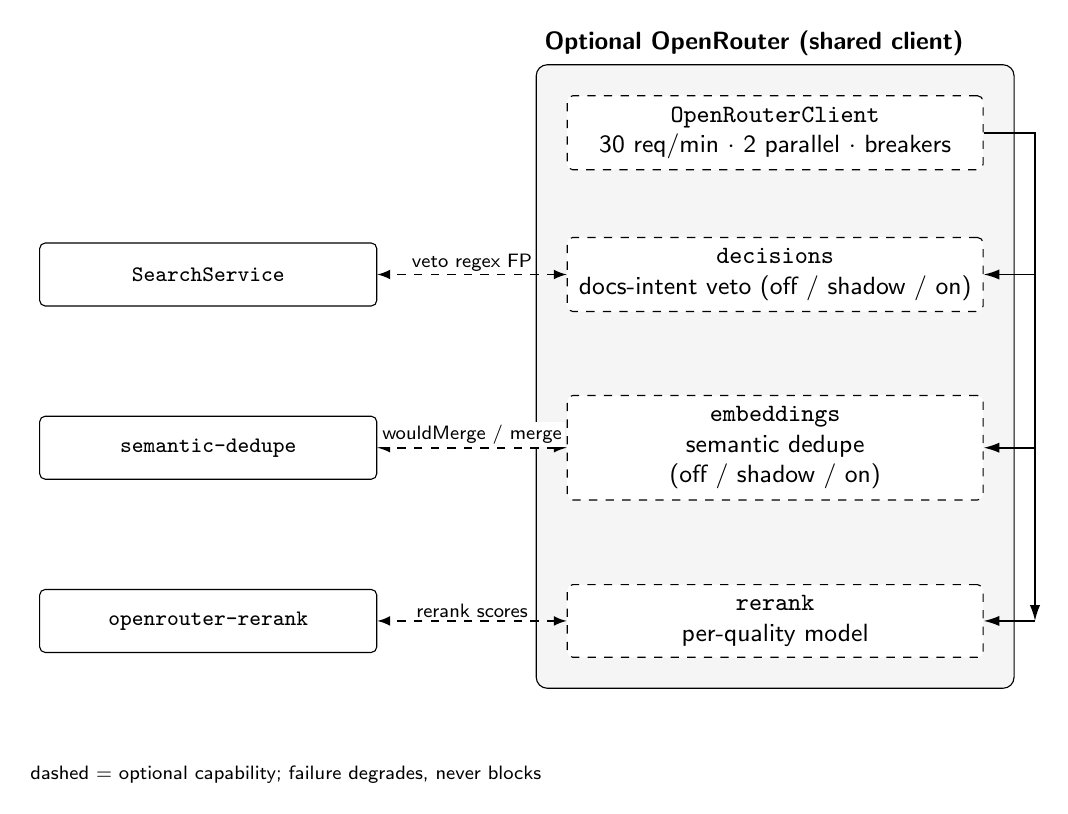
\begin{tikzpicture}
\node[optbox] (orc) at (0,5.2) {\texttt{OpenRouterClient}\\30 req/min $\cdot$ 2 parallel $\cdot$ breakers};
\node[optbox] (dec) at (0,3.4) {\texttt{decisions}\\docs-intent veto (off / shadow / on)};
\node[optbox] (emb) at (0,1.2) {\texttt{embeddings}\\semantic dedupe (off / shadow / on)};
\node[optbox] (rer) at (0,-1.0) {\texttt{rerank}\\per-quality model};

\node[target] (tsvc) at (-7.2,3.4) {\texttt{SearchService}};
\node[target] (tsem) at (-7.2,1.2) {\texttt{semantic-dedupe}};
\node[target] (trer) at (-7.2,-1.0) {\texttt{openrouter-rerank}};

\draw[arrow] (orc.east) -- (3.3,5.2) -- (3.3,-1.0);
\draw[arrow] (3.3,3.4) -- (dec.east);
\draw[arrow] (3.3,1.2) -- (emb.east);
\draw[arrow] (3.3,-1.0) -- (rer.east);

\draw[ddbl] (dec.west) -- node[lbl,above] {veto regex FP} (tsvc.east);
\draw[ddbl] (emb.west) -- node[lbl,above] {wouldMerge / merge} (tsem.east);
\draw[ddbl] (rer.west) -- node[lbl,above] {rerank scores} (trer.east);

\begin{scope}[on background layer]
  \node[frame, fit=(orc)(rer)] (panel) {};
\end{scope}
\node[ftitle] at ([xshift=2pt,yshift=2pt]panel.north west) {Optional OpenRouter (shared client)};

\node[lbl, anchor=north west, fill=none] at (-9.5,-2.8) {dashed = optional capability; failure degrades, never blocks};
\end{tikzpicture}
\end{document}